\documentclass[english]{scrartcl}
\usepackage[T1]{fontenc}
\usepackage[utf8]{inputenc}
\usepackage[scaled=.8]{beramono}
\usepackage{geometry}
\geometry{verbose,tmargin=3cm,bmargin=3cm,lmargin=3cm,rmargin=3cm}
\usepackage{microtype}
\usepackage[parfill]{parskip}
\usepackage{amsmath}
\usepackage{graphicx}
\usepackage{hyperref}
\usepackage{nameref}
\usepackage{float}
\usepackage{listings}
\usepackage{color}
\usepackage{fancyhdr}
\usepackage{blindtext}

\pagestyle{fancy}
\fancyhf{}
\rhead{A Team}
\lhead{CC: PaaS}
\cfoot{\thepage}

\newcommand*{\fullref}[1]{\hyperref[{#1}]{\autoref*{#1}~\nameref*{#1}}}

\definecolor{darkgray}{rgb}{0.66, 0.66, 0.66}
\definecolor{asparagus}{rgb}{0.53, 0.66, 0.42}

\lstdefinestyle{s}{
  commentstyle=\color{darkgray},
  keywordstyle=\bfseries,
  morekeywords={},
  stringstyle=\color{asparagus},
  basicstyle=\ttfamily\footnotesize,
  breakatwhitespace=false,
  keepspaces=true,
  numbersep=5pt,
  showspaces=false,
  showstringspaces=false,
}

\lstset{style=s}

\begin{document}

\title{Cloud Computing\\PaaS: Web Crawler}

\author{Sonja Biedermann \and Augusto Jose de Oliveira Martins \and Tobias Harald Herbert}

\maketitle
\tableofcontents

\section{Project Description}

\section{Implementation}

We decided to implement the project using Python3. Our cloud platform of choice
is AWS. The only dependencies the project has are

\begin{itemize}
    \item \texttt{requests}, for issuing HTTP requests,
    \item \texttt{validators}, for validating URLs, and
    \item \texttt{boto3}, the AWS SDK for Python.
\end{itemize}

We use DynamoDB for storage and SQS for message passing. The workers are realized
as AWS Lambda functions. The master can be deployed using ElasticBeanstalk (AWS'
traditional PaaS offering), which in turn uses Autoscaling, S3, Load Balancing
and monitoring automatically, although this is not needed---the traffic on the
master is very low.

The implementation can be found \href{https://github.com/biederfrau/cloud-computing-paas}{on GitHub}.

\subsection{Frontend}

The frontend is a simple one-page website which communicates with the
master node running on EC2 and displays data derived from the crawl and
information about the current state of the crawler.

We display how many workers are currently working on the task. Since we use AWS
Lambda, whose functions are quite short-lived, this chart sees a lot of
activity with workers popping in and out of existence. The purpose of this
chart is to ``visualize the cloud'' and see how it scales.

The result of the crawl is displayed as a network. Nodes are colored according
to the host, however note that colors may be repeated. To draw the network, we
use the constraint-based layout algorithm
CoLa\footnote{\url{https://ialab.it.monash.edu/webcola/}}, which basically runs
a small simulation and optimizes the layout. The results from this algorithm
are excellent, but graph drawing is hard and as a consequence we limit the
graph display to 500 edges. The performance is heavily dependent on the graph
structure, e.g. networks with very fat hubs (e.g. Wikipedia) have noticeably
worse performance than networks with many smaller hubs. This is due to how
large the neighborhoods tend to be in the hubs vicinity. It also does not help
that it is running in the browser.

The graph is interactive and allows you to drag the nodes around should
you not be satisfied with the layout. You can also click on a node to
visit the associated webpage.

Figure~\ref{fig:screenshot} shows the result of a crawl on the webpage of an
ongoing research project. The graph shows 4 hubs: reddit (red), arXiv (green),
Wikipedia (orange), and the web presence of the University of California in Riverside
(blue), which is split between two involved researchers.

The bottom displays the current number of discovered edges, which is equivalent
to the amount of pages crawled, as well as the current depth. Do note that the
typical web page has an extremely high fan out at depths of about 3 to 4, so
the time spent at consecutive depths grows exponentially. We have thus not
opted to display this as a progress bar, since the rate of progress is hard to
estimate.

\begin{figure}
    \centering
    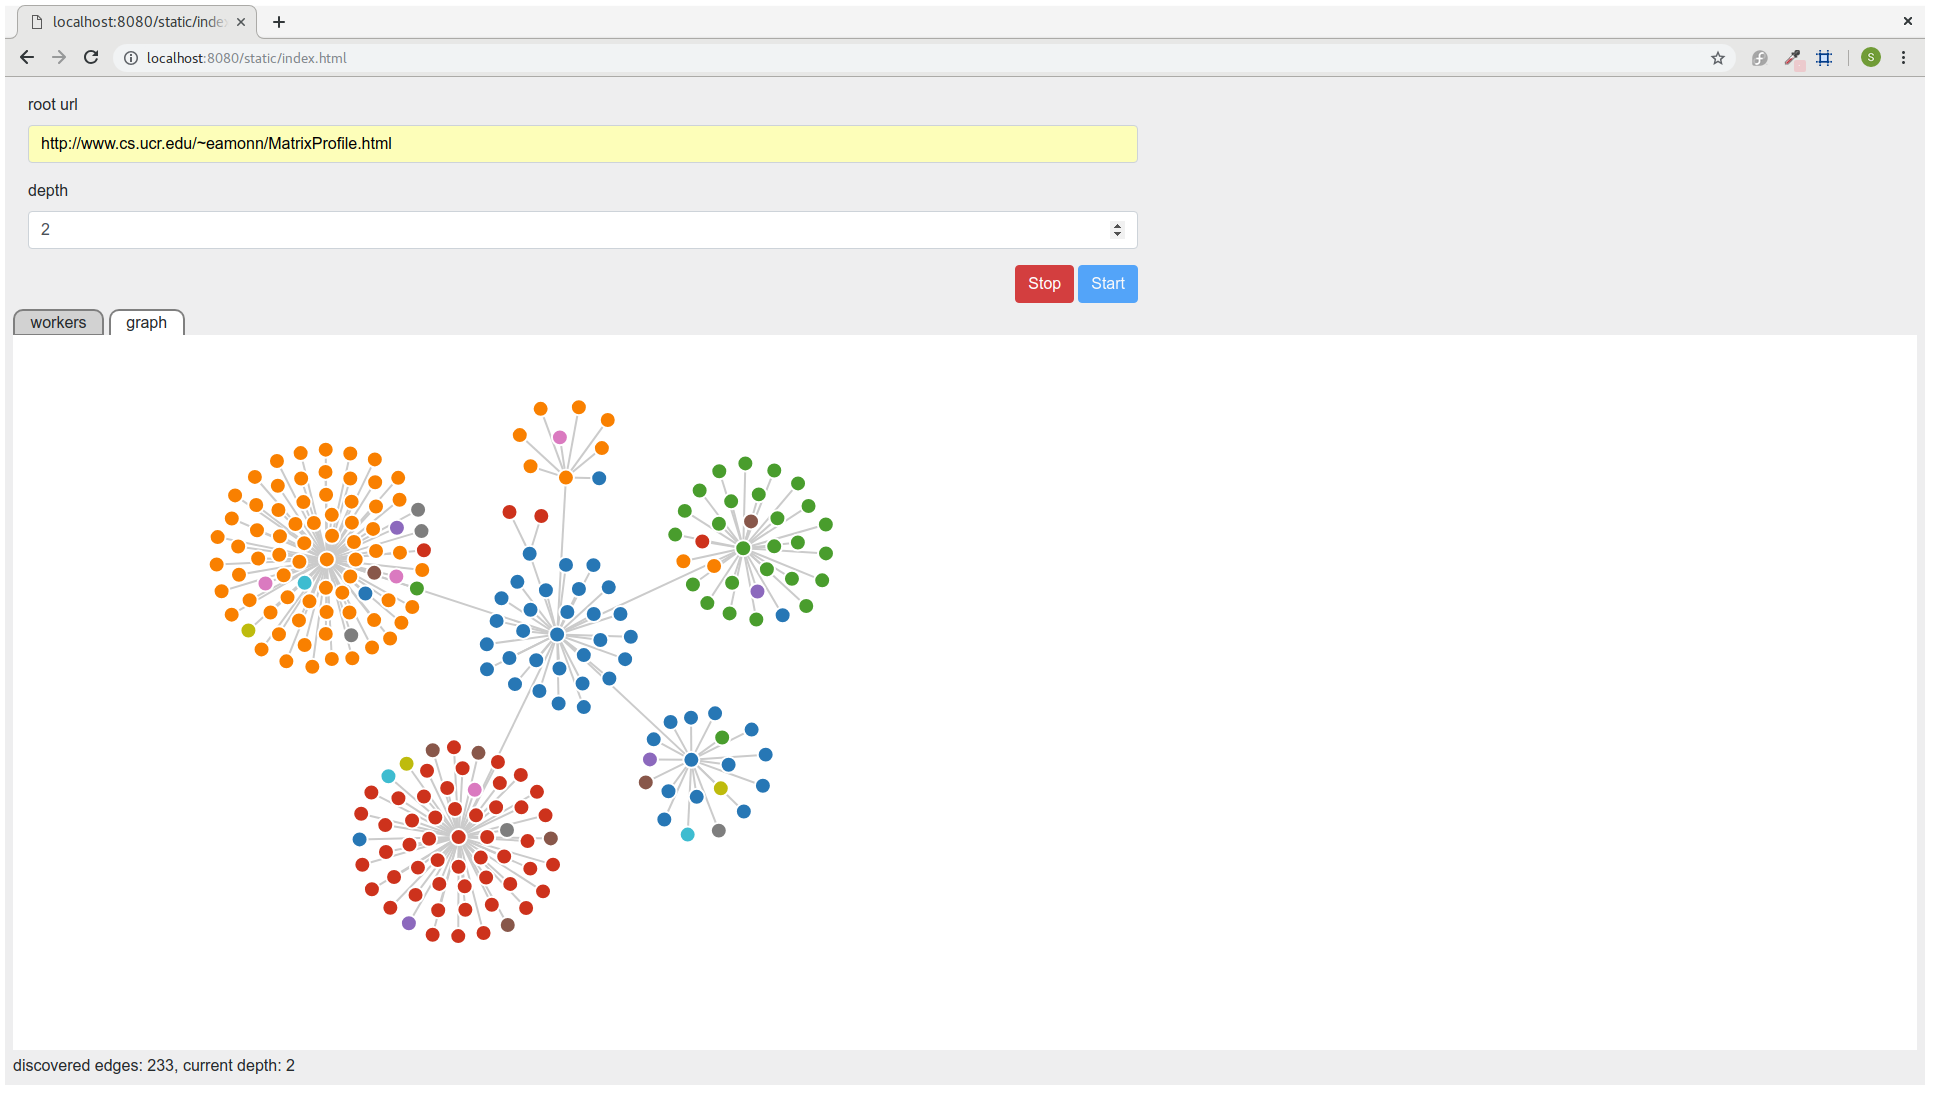
\includegraphics[width=\textwidth]{img/screenshot}
    \caption{Screenshot of the graph view}
    \label{fig:screenshot}
\end{figure}

\subsection{Backend}

\subsubsection{Master}

The master runs a lightweight web server (using
\href{https://bottlepy.org/docs/dev/}{Bottle}, a micro WSGI web framework)
serving the frontend and offers a small REST API for querying the state of the
crawl. This basically consists of starting the crawl and querying the workers
and discovered edges.

The master can be deployed to an EC2 instance using ElasticBeanstalk or run
locally.

\subsubsection{Worker}

\section{Setup}

We have included setup scripts in \texttt{setup}. They create all resources
used and also set up the needed policies. % make it so this sentence is true

\subsection{Master}

You can either run the master locally using the \texttt{master.py} contained
in the project root. It serves on port 8080.

If you want to deploy it via ElasticBeanstalk, do the following at project
root:

\begin{verbatim}
$ cd eb_master
$ make
\end{verbatim}

The Makefile copies the files properly, runs the EB CLI commands to get
everything ready, attaches the needed policies to your user and also the EC2
instance role which will run the application, and then launches the application
in your default browser. We presume that the AWS and EB CLI are installed and
set up properly.

Once the master is up and running, you can deploy the worker as described in
the next section. The ordering between master and worker is not actually
important.

To terminate the EC2 instance and clean up the files run \texttt{make clean}
later. Please be aware that deletion will take a bit to take effect. Also, the
output tells you that it is fine to Ctrl+C, but don't---while interrupting the
EB CLI (who produces the output) is fine, interrupting \texttt{make} is not.

\subsection{Worker(s)}

\end{document}
